\let\negmedspace\undefined
\let\negthickspace\undefined
\documentclass[journal]{IEEEtran}
\usepackage[a5paper, margin=10mm, onecolumn]{geometry}
%\usepackage{lmodern} % Ensure lmodern is loaded for pdflatex
\usepackage{tfrupee} % Include tfrupee package

\setlength{\headheight}{1cm} % Set the height of the header box
\setlength{\headsep}{0mm}     % Set the distance between the header box and the top of the text

\usepackage{gvv-book}
\usepackage{gvv}
\usepackage{cite}
\usepackage{amsmath,amssymb,amsfonts,amsthm}
\usepackage{algorithmic}
\usepackage{graphicx}
\usepackage{textcomp}
\usepackage{xcolor}
\usepackage{txfonts}
\usepackage{listings}
\usepackage{enumitem}
\usepackage{mathtools}
\usepackage{gensymb}
\usepackage{comment}
\usepackage[breaklinks=true]{hyperref}
\usepackage{tkz-euclide} 
\usepackage{listings}
% \usepackage{gvv}                                        
\def\inputGnumericTable{}                                 
\usepackage[latin1]{inputenc}                                
\usepackage{color}                                            
\usepackage{array}                                            
\usepackage{longtable}                                       
\usepackage{calc}                                             
\usepackage{multirow}                                         
\usepackage{hhline}                                           
\usepackage{ifthen}                                           
\usepackage{lscape}
\begin{document}

\bibliographystyle{IEEEtran}
\vspace{3cm}
\title{1.1.5.7}
\author{EE24BTECH11008 - Aslin Garvasis
}
% \maketitle
% \newpage
% \bigskip
{\let\newpage\relax\maketitle}

\renewcommand{\thefigure}{\theenumi}
\renewcommand{\thetable}{\theenumi}
\setlength{\intextsep}{10pt} % Space between text and floats


\numberwithin{equation}{enumi}
\numberwithin{figure}{enumi}
\renewcommand{\thetable}{\theenumi}
 \textbf{Question:}If $\vec{A}(\frac{a}{3},4)$ is the midpoint of the line segment joining the points $\vec{B}(-6,5)$ and $\vec{C}(-2,3),$  
		then the value of $a$ is\\
 
 \solution As $\vec{A}$ is the midpoint of $\vec{B}$ and $\vec{C}$, $\vec{A}$ can be represented as \\ 
		$$\vec{A}=\frac{\vec{B}+\vec{C}}{2}$$ \\
		
		$$\vec{A}=\frac{\myvec{-6\\5}+\myvec{-2\\3}}{2}=\frac{\myvec{-8\\8}}{2}=\myvec{-4\\4}$$
		also, $$\vec{A}=\myvec{\frac{a}{3}\\4}$$\\
  \begin{align}
      \implies a&=-4\times3=-12
  \end{align}
		\newpage


		\begin{figure}[h!]
                \centering
               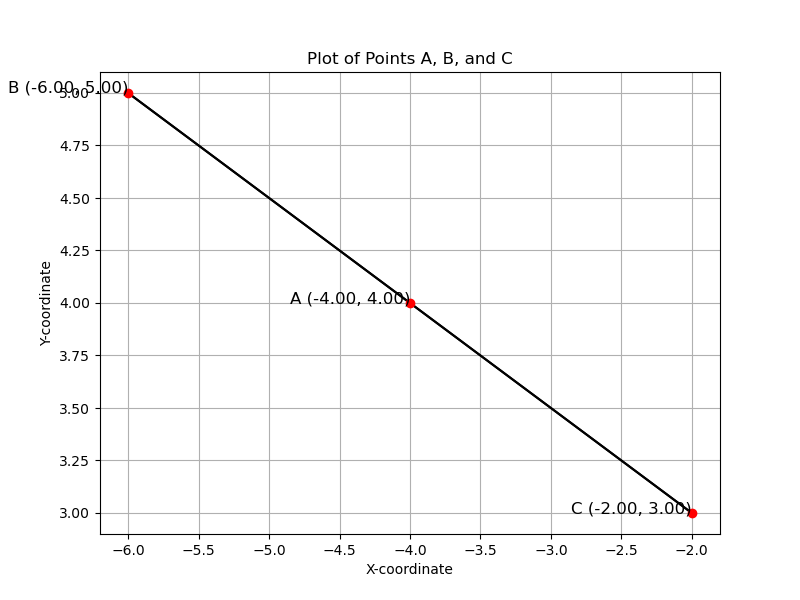
\includegraphics[width=0.7\linewidth]{figs/Fig1.png}
			\caption{Plot of points $\vec{A}$, $\vec{B}$ and $\vec{P}$}
               \label{stemplot}
               \end{figure}
\end{document}
